\documentclass[12pt]{article}

\setlength{\textwidth}{17cm}
\setlength{\textheight}{24cm}
\setlength{\topmargin}{-2cm}
\setlength{\footskip}{1cm}
\setlength{\evensidemargin}{0cm}
\setlength{\oddsidemargin}{0cm}
\setlength{\parindent}{0cm}


\usepackage{amsmath}
\usepackage[magyar]{babel}
\usepackage[T1]{fontenc}
\usepackage[utf8]{inputenc}
\usepackage{fixltx2e}
\usepackage{multirow}
\usepackage{hyperref}
\usepackage{graphicx}
%\usepackage{gensymb}
\usepackage{float}

\begin{document}

%itt lesz a gorbe
A Lorentz-görbe a következő alakú:
\[  f(x) = \frac{a}{(1+s(x-x_0)^2)}\]
Ennek deriváltja
\[ \frac{df}{dx} = \frac{-2as(x-x_0)}{(1+s(x-x_0)^2)^2}\]

\begin{figure}[H]
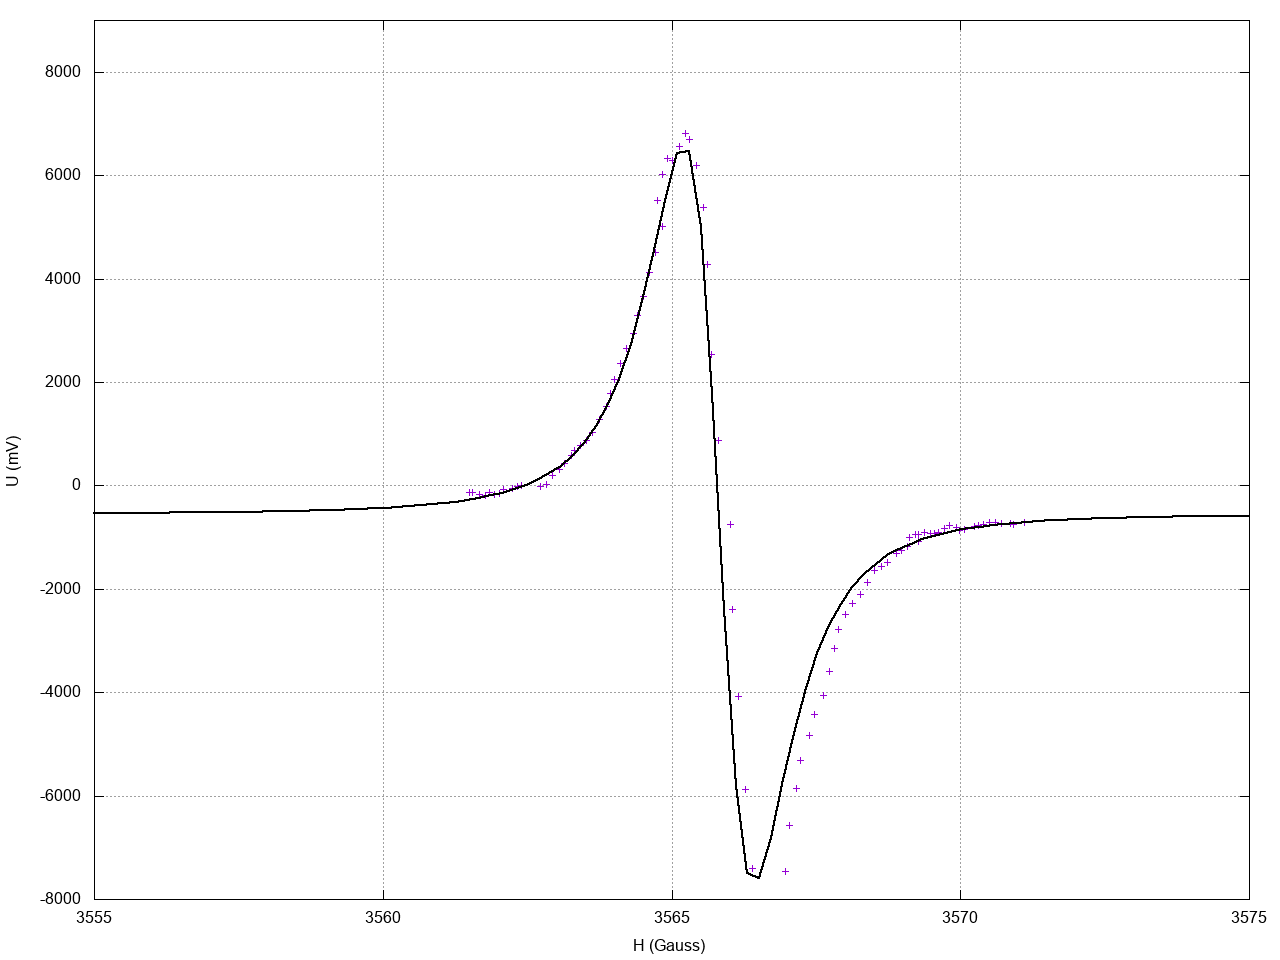
\includegraphics[width=15cm]{cr6.png}
\centering
\caption{A mérési adatok, és az illesztett derivált Lorentz-görbe Cr minta esetén}
\label{fig:3}
\end{figure}

\begin{figure}[H]
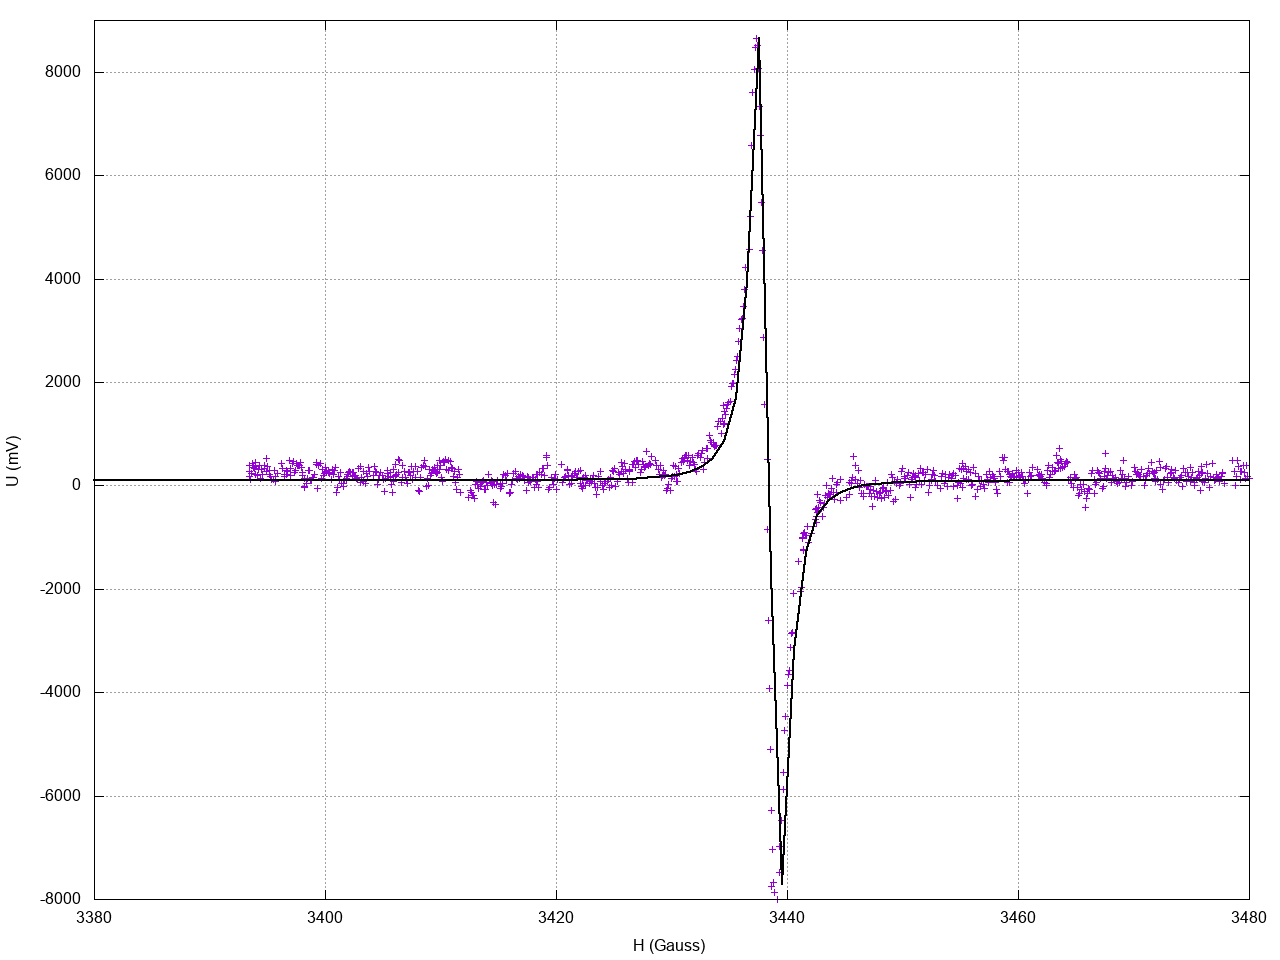
\includegraphics[width=15cm]{mn.png}
\centering
\caption{A mérési adatok, és az illesztett derivált Lorentz-görbe Mn minta esetén}
\label{fig:4}
\end{figure}

\begin{center}
\begin{table}[H]
\begin{tabular}{|c|c|c|c|c|c|c|c|}
 \hline
$a$ & $s$ & $x_0$ & $c$ \\ \hline
$12930$ & $0.812$ & $3225$ & $-50$ \\ \hline
$12930$ & $0.889$ & $3290.4$ & $-154$ \\ \hline
$11930$ & $0.989$ & $3357.2$ & $-284$ \\ \hline
$13050$ & $0.783$ & $3425.36$ & $-284$ \\ \hline
$11924$ & $1.005$ & $3495.02$ & $-104$ \\ \hline
$11524$ & $0.9105$ & $3565.82$ & $-554$ \\ \hline
\end{tabular}
\caption{A $Cr$-minta esetében mért ESR jelre illesztett görbe paraméterei}
\label{tab:1}
\end{table}
\end{center}

\begin{center}
\begin{table}[H]
\begin{tabular}{|c|c|c|c|c|c|c|c|}
 \hline
$a$ & $s$ & $x_0$ & $c$ \\ \hline
$17524$ & $0.6105$ & $3438.5$ & $100$ \\ \hline
\end{tabular}
\caption{A $Mn$-minta esetében mért ESR jelre illesztett görbe paraméterei}
\label{tab:2}
\end{table}
\end{center}

\end{document}
